\pdfminorversion=4  % Acrobat 5.0 / PDF 1.4 compatibility (IEEE camera-ready PDF settings)
\documentclass[conference]{IEEEtran}
\IEEEoverridecommandlockouts

\usepackage{cite}
\usepackage{amsmath,amssymb,amsfonts}
% \usepackage{algorithmic}  % unused; not in a base TeX Live install (texlive-science)
% \usepackage{algorithm}    % unused
\usepackage{graphicx}
\usepackage{textcomp}
\usepackage{xcolor}
\usepackage{tikz}
\usetikzlibrary{shapes.geometric}
\usepackage{pgfplots}
\pgfplotsset{compat=1.18}
\usepgfplotslibrary{groupplots}
\usepackage{booktabs}
\usepackage{multirow}
\usepackage{url}
\usepackage{stfloats}
\usepackage[hidelinks]{hyperref}  % clickable links (code URL), no coloured boxes

\def\BibTeX{{\rm B\kern-.05em{\sc i\kern-.025em b}\kern-.08em
    T\kern-.1667em\lower.7ex\hbox{E}\kern-.125emX}}

\begin{document}

\title{ApproxDA-TransUNet: Understanding Global Context Sensitivity of Attention Approximation for Medical Image Segmentation\thanks{\IEEEauthorrefmark{1}Corresponding author.}}

\author{
\IEEEauthorblockN{Jiawei Zhong}
\IEEEauthorblockA{\textit{DeepSOTA AI}\\
San Jose, United States\\
deepsota.ai@gmail.com}
\and
\IEEEauthorblockN{Qin Chen}
\IEEEauthorblockA{\textit{Shenzhen Cloudage Technology Ltd.}\\
Shenzhen, China\\
chenqin0773@hotmail.com}
\and
\IEEEauthorblockN{Hui Zhang\IEEEauthorrefmark{1}}
\IEEEauthorblockA{\textit{College of Information, Mechanical}\\
\textit{and Electrical Engineering}\\
\textit{Shanghai Normal University}\\
Shanghai, China\\
huiz@shnu.edu.cn}
}

\maketitle

% !TEX root = ../ApproxDA-TransUNet.tex
\begin{abstract}
Dual-attention mechanisms have demonstrated strong performance in medical image segmentation by jointly modeling long-range spatial and channel dependencies, yet their quadratic complexity has motivated numerous approximation strategies whose task-dependent behavior remains poorly understood. To investigate this, we propose Approximate Dual Attention TransUNet (ApproxDA-TransUNet), a dual-attention approximation framework for hybrid CNN-Transformer architectures that integrates controllable windowed low-rank spatial attention with grouped channel attention. Beyond serving as an efficiency mechanism, ApproxDA-TransUNet provides a parametric platform to systematically evaluate how attention approximation interacts with representation capacity across diverse clinical segmentation tasks.
On Synapse Multi-Organ CT, CVC-ClinicDB polyp, and ISIC 2018 skin lesion benchmarks, ApproxDA-TransUNet achieves 81.63\%, 90.54\%, and 89.26\% Dice, improving Dice over the reported DA-TransUNet results on all three datasets. Furthermore, our empirical analysis reveals two key insights. First, window sensitivity varies markedly across tasks: the Dice spread across window sizes is up to 3.5$\times$ larger on multi-organ CT than on polyp and lesion targets, a characteristic we formalize as empirical Global Context Sensitivity (GCS). Second, in our multi-organ CT experiments, the learnable routing gate stayed near uniform blending and did not outperform single-branch routing. These findings indicate that the best attention-approximation configuration is task-dependent rather than universal.
\end{abstract}

\begin{IEEEkeywords}
medical image segmentation, dual attention, attention approximation, window size, global context sensitivity
\end{IEEEkeywords}

% !TEX root = ../ApproxDA-TransUNet.tex
\section{Introduction}

Transformers have advanced medical image segmentation by enabling global long-range dependency modeling that convolutional networks capture only indirectly. Dual attention~\cite{fu2019dual}---combining a Position Attention Module (PAM) for spatial correlations and a Channel Attention Module (CAM) for channel correlations---has emerged as a powerful mechanism, and methods such as DA-TransUNet~\cite{sun2024datransunet} demonstrated its effectiveness in hybrid CNN-Transformer architectures for multi-organ and polyp segmentation. The quadratic complexity of dual attention, however, has prompted a wave of efficient approximations---windowed attention~\cite{liu2021swin}, low-rank factorization~\cite{wang2020linformer}, and grouped channel interaction~\cite{rahman2024emcad}---that are now standard design choices. These strategies are usually adopted under the implicit assumption that approximation is broadly applicable with minor accuracy trade-offs---an assumption rarely examined across tasks with different spatial characteristics:

\begin{center}
\emph{When, and at what scale, is attention approximation\\
beneficial for medical image segmentation?}
\end{center}
To investigate this question, we design \textbf{ApproxDA-TransUNet}\footnote{Code: \url{https://github.com/deepsota-ai/ApproxDA-TransUNet}}: a dual-attention architecture featuring three independently controllable approximation axes---windowed PAM, low-rank projection, and grouped CAM. ApproxDA-TransUNet provides both competitive segmentation performance across benchmarks and a controllable framework for studying the spatial and channel granularity of attention.

Applying ApproxDA-TransUNet across three medical segmentation benchmarks reveals distinct task-dependent characteristics: the windowed attention operator is most window-sensitive on multi-organ CT and less so on polyp and skin lesion segmentation. With an appropriately selected window, ApproxDA-TransUNet improves Dice on all three benchmarks over the reported DA-TransUNet results, while showing that sensitivity to the context window differs across clinical targets. We further observe that, on multi-organ CT, learnable routing between spatial and channel branches stays at near-uniform weighting without surpassing single-branch routing.

The main contributions of this paper are:

\begin{itemize}

\item \textbf{ApproxDA-TransUNet Framework}: We propose ApproxDA-TransUNet, a dual-attention approximation architecture featuring three independently parameterizable operators---windowed PAM, low-rank projection, and grouped CAM---improving Dice over the reported DA-TransUNet results on three diverse benchmarks.

\item \textbf{Systematic Context Sensitivity Study}: Using ApproxDA-TransUNet as a controlled diagnostic platform, we present a systematic empirical study of attention approximation across heterogeneous medical segmentation tasks, observing up to a 3.5$\times$ difference in window sensitivity across benchmarks. We formalize this behavior via an empirical \emph{Global Context Sensitivity (GCS)} metric, quantifying the architectural response to window scale across distinct anatomical targets.

\item \textbf{Empirical Insights on Approximation and Routing}: We find that exact attention shows no consistent advantage over its low-rank approximation, and document that learnable dual-branch routing stays at near-uniform fusion on multi-organ CT without surpassing single-branch routing.

\end{itemize}

The remainder of this paper is organized as follows: Section~\ref{sec:related_work} reviews related work; Section~\ref{sec:method} presents the ApproxDA-TransUNet framework; Section~\ref{sec:experiments} compares it with published methods; Section~\ref{sec:understanding} reports ablation studies and analysis; Section~\ref{sec:conclusion} concludes.

% !TEX root = ../ApproxDA-TransUNet.tex
\section{Related Work}
\label{sec:related_work}

\subsection{CNN-based Medical Image Segmentation}

Convolutional encoder-decoder architectures established the foundational paradigm for medical image segmentation, with U-Net~\cite{ronneberger2015unet} introducing the skip-connection design that underpins most segmentation networks, and successors~\cite{zhou2018unetpp,oktay2018attention,diakogiannis2020resunet,ibtehaz2020multiresunet} progressively adding dense connections, attention gating, and residual learning for improved feature reuse and training stability. These models offer strong computational efficiency and are well suited to local texture patterns, but their fixed receptive fields cannot capture long-range spatial dependencies across anatomical structures, limiting performance on tasks requiring global context.

\subsection{Transformer-based Medical Image Segmentation}

Transformer architectures have significantly advanced medical image segmentation by enabling global dependency modeling beyond the locality of convolutional neural networks. Representative methods such as TransUNet~\cite{chen2021transunet}, Swin-Unet~\cite{cao2022swinunet}, UNETR~\cite{hatamizadeh2022unetr}, UCTransNet~\cite{wang2022uctransnet}, TransNorm~\cite{azad2022transnorm}, and DAEformer~\cite{azad2023daeformer} combine convolutional feature extraction with transformer-based contextual modeling and report strong segmentation performance across a wide range of medical imaging tasks. These methods treat global context modeling as uniformly beneficial, however, without examining whether different tasks require different degrees of spatial context.

\subsection{Dual Attention and DA-TransUNet}

DANet~\cite{fu2019dual} introduced Position Attention Modules (PAM) and Channel Attention Modules (CAM), capturing spatial and channel correlations at $\mathcal{O}(N^2C)$ and $\mathcal{O}(C^2N)$ complexity respectively. DA-TransUNet~\cite{sun2024datransunet} adapted this design for medical image segmentation by inserting dual-attention blocks at multiple skip connections of a hybrid R50-ViT-B/16 encoder-decoder, improving accuracy while inheriting the quadratic cost of full-map attention. DBAANet~\cite{li2025dbaanet} further extends dual-branch attention by aggregating position and channel attention across multiple scales, demonstrating the continued appeal of dual-attention paradigms for medical image segmentation.

\subsection{Efficient Attention and Adaptive Routing}

Windowed local attention~\cite{liu2021swin}, low-rank projection~\cite{wang2020linformer}, and grouped channel interaction~\cite{rahman2024emcad} have become standard strategies for reducing the computational footprint of global attention, with learnable gating widely adopted to blend multi-branch representations~\cite{azad2023daeformer,rahman2024emcad}. DAMamba~\cite{ding2025damamba} further demonstrates that dual-attention routing transfers effectively to state-space models for lightweight breast ultrasound segmentation, highlighting the versatility of multi-branch attention paradigms. While existing efficient attention methods are predominantly evaluated by computational metrics, their task-dependent impact on feature representation and segmentation accuracy remains under-explored. In this work, we systematically investigate this interaction by varying approximation parameters across diverse clinical tasks and evaluating the empirical behavior of adaptive branch routing.
% !TEX root = ../ApproxDA-TransUNet.tex
\section{Method}
\label{sec:method}

This section introduces the overall architecture of ApproxDA-TransUNet and the placement of ApproxDABlocks within it, details the three independently controllable approximation axes implemented in each block, and analyzes their computational characteristics.

\subsection{Architecture Overview}

Figure~\ref{fig:framework} illustrates the overall architecture: ApproxDA-TransUNet adopts the hybrid CNN--ViT encoder-decoder structure of DA-TransUNet~\cite{sun2024datransunet}, with an R50-ViT-B/16 backbone pretrained on ImageNet-21K. Three CNN encoder stages produce features at $112{\times}112$, $56{\times}56$, and $28{\times}28$ resolutions (strides 2, 4, and 8 for a $224{\times}224$ input), while a 12-layer ViT processes $14{\times}14$ patch tokens at the bottleneck. While DA-TransUNet integrates attention modules at three stages (the bottleneck and the 512- and 256-channel skip paths), ApproxDA-TransUNet uniformly equips all three skip connections (512 channels at $28{\times}28$, 256 at $56{\times}56$, and 64 at $112{\times}112$) as well as the bottleneck (768 channels at $14{\times}14$) with ApproxDABlocks, providing multi-scale context modulation. Each ApproxDABlock keeps the DANetHead layout of DA-TransUNet and only replaces its attention operators: each branch first compresses the $C$ input channels to $C' {=} C/16$ with a $3{\times}3$ convolution, batch normalization and ReLU, applies the approximated attention, and refines the result with a second $3{\times}3$ convolution--BN--ReLU. A Low-Rank Windowed PAM branch and a Grouped CAM branch are fused via a configurable gating vector $\mathbf{g}$ and projected back to $C$ channels. Figure~\ref{fig:approxda_block} details the internal structure of the ApproxDABlock and its three parameterized approximation axes.

\begin{figure*}[tbp]
  \centering
  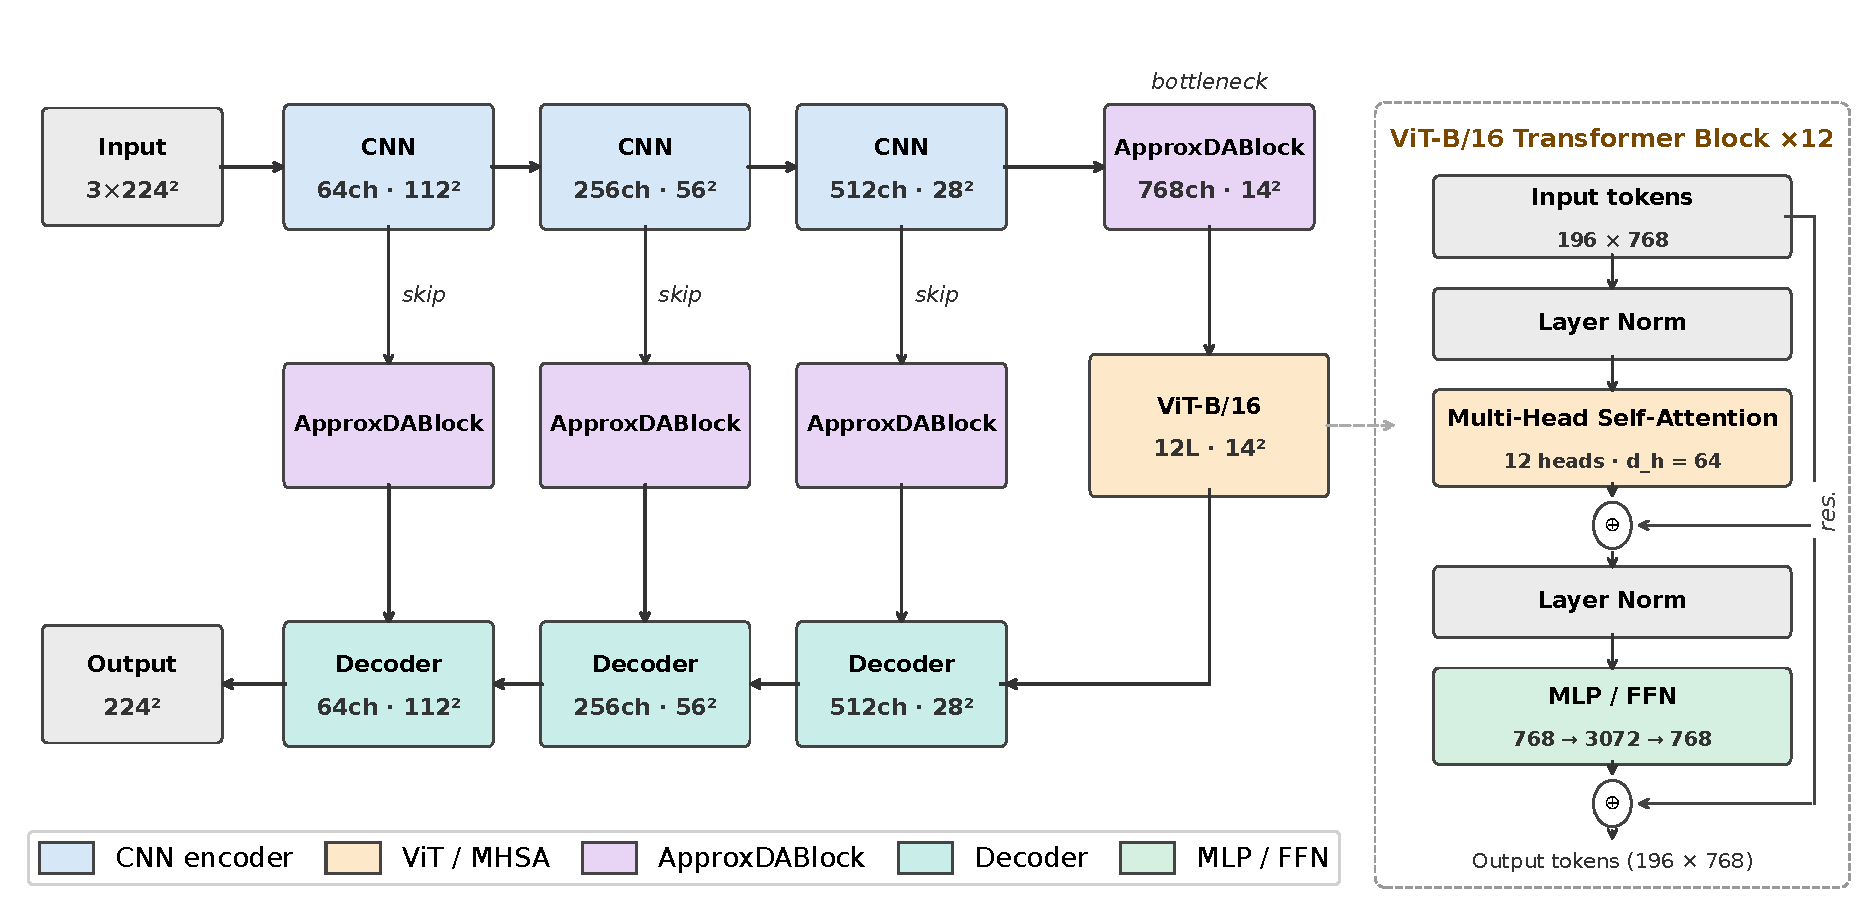
\includegraphics[width=\textwidth]{figures/approxda_overview}
  \caption{ApproxDA-TransUNet architecture. ApproxDABlocks are placed at the bottleneck and at all three skip connections.}
  \label{fig:framework}
\end{figure*}

% figures/approxda_block.pdf is generated by PlotNeuralNetScripts/approxda_block.py
\begin{figure*}[tbp]
  \centering
  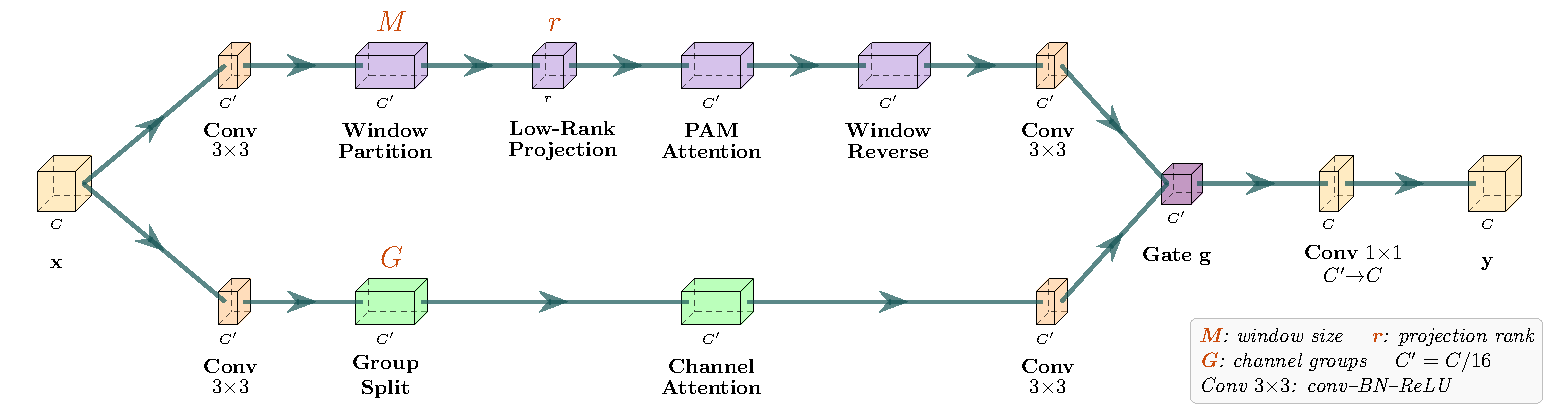
\includegraphics[width=\textwidth]{figures/approxda_block}
  \caption{ApproxDABlock with its three approximation axes $M$, $r$ and $G$. Upper branch: Low-Rank Windowed PAM; lower branch: Grouped CAM.}
  \label{fig:approxda_block}
\end{figure*}

\subsection{Attention Approximation Formulation}

Standard dual attention performs dense spatial and channel affinity modeling over the entire feature map, incurring quadratic complexity in both spatial resolution and channel count. ApproxDA-TransUNet structures this complexity along three orthogonal axes, each governing a distinct dimension of the approximation:

\textbf{Spatial scope} (window size $M$) controls the receptive range of spatial attention. Full global attention ($M{=}H$) models all pairwise spatial dependencies, whereas local $M{\times}M$ window partitioning restricts attention to local neighborhoods at reduced complexity.

\textbf{Representation fidelity} (rank $r$) controls the subspace precision within each window. Low-rank projection ($r \ll M^2$) compresses the key--value affinity matrix into an informative subspace, while higher $r$ approaches exact intra-window attention.

\textbf{Channel interaction} (groups $G$) controls the cross-channel dependency span in CAM. Partitioning $C$ channels into $G$ independent groups constrains channel correlations to within-group interactions, scaling the interaction granularity.

Because these parameters are orthogonally parameterized, any element in $\{M,\,r,\,G\}$ can be independently ablated while maintaining the others constant.

\subsection{Spatial Approximation}

Instead of computing global position attention, ApproxDA-TransUNet partitions the feature map into non-overlapping windows of size $M{\times}M$. Attention is computed independently inside each local window, reducing complexity from $\mathcal{O}(N^2C)$ to $\mathcal{O}(NM^2C)$, where $N = HW$.

\textbf{Window partitioning.} Following~\cite{liu2021swin}, we partition the compressed $C'{\times}H{\times}W$ feature map into $n_W$ non-overlapping $M{\times}M$ windows, with $M \leftarrow \min(M, H, W)$. For one window, let $\mathbf{X} \in \mathbb{R}^{C' \times N_w}$ with $N_w = M^2$ denote its features, and let
\begin{equation}
\begin{aligned}
  \mathbf{Q} = \mathbf{W}_Q\mathbf{X},\; \mathbf{K} &= \mathbf{W}_K\mathbf{X} \in \mathbb{R}^{C_q \times N_w}, \\
  \mathbf{V} &= \mathbf{W}_V\mathbf{X} \in \mathbb{R}^{C' \times N_w}
\end{aligned}
  \label{eq:qkv}
\end{equation}
be the query, key, and value features produced by $1{\times}1$ convolutions (with bias), where $C_q = \max(1, C'/8)$ as in DA-TransUNet's PAM.

\textbf{Low-rank projection.} Following~\cite{wang2020linformer}, keys and values inside each window are compressed along the token axis by a learned projection $\mathbf{P} \in \mathbb{R}^{N_w \times r}$, shared by keys and values and across windows within a block:
\begin{equation}
  \tilde{\mathbf{K}} = \mathbf{K}\mathbf{P} \in \mathbb{R}^{C_q \times r}, \quad \tilde{\mathbf{V}} = \mathbf{V}\mathbf{P} \in \mathbb{R}^{C' \times r}.
  \label{eq:lowrank}
\end{equation}
Each of the $N_w$ queries attends to the $r$ projected keys:
\begin{equation}
\begin{aligned}
  \mathbf{A} &= \operatorname{softmax}\!\big(\mathbf{Q}^{\top}\tilde{\mathbf{K}}\big) \in \mathbb{R}^{N_w \times r}, \\
  \mathbf{E} &= \alpha\,\big(\mathbf{A}\tilde{\mathbf{V}}^{\top}\big)^{\!\top} + \mathbf{X} \in \mathbb{R}^{C' \times N_w},
\end{aligned}
  \label{eq:pam_lr}
\end{equation}
where the softmax normalizes each row across the $r$ projected keys, without temperature scaling (consistent with standard PAM~\cite{fu2019dual}), and $\alpha$ is a learned scalar initialized to 0. Each window output $\mathbf{E}$ is reshaped to $C'{\times}M{\times}M$, and all windows are reassembled into the $H{\times}W$ grid. Setting $r{=}0$ removes the projection ($\tilde{\mathbf{K}}{=}\mathbf{K}$, $\tilde{\mathbf{V}}{=}\mathbf{V}$), giving exact attention inside each window; with $r{=}0$, $M \geq H, W$ and $G{=}1$, the block reduces to DA-TransUNet's DANetHead. The full $N_w{\times}N_w$ affinity is thus substituted by an $N_w{\times}r$ matrix, lowering attention complexity to $\mathcal{O}(NrC)$. When $M$ is clamped to match feature dimensions, the leading $N_w$ rows of $\mathbf{P}$ are utilized; setting $M{=}112$ establishes global spatial scope per feature map while preserving low-rank ($r{=}32$) projection. Together, windowing and low-rank projection reduce the theoretical attention-matrix complexity from $\mathcal{O}(N^2)$ to $\mathcal{O}(Nr)$ (${\sim}390{\times}$ reduction in affinity matrix entries at $112{\times}112$ with $r{=}32$; see Section~\ref{sec:efficiency}).

\subsection{Channel Approximation}

The standard Channel Attention Module computes a full $C'{\times}C'$ channel correlation matrix at $\mathcal{O}(C'^2N)$ complexity. ApproxDA-TransUNet approximates this by partitioning the $C'$ compressed channels into $G$ groups of width $C_g = C'/G$ (with $G \leftarrow \min(G, C')$) and computing independent per-group attention. For group $g$ with channel slices $\mathbf{A}^{(g)}_1, \dots, \mathbf{A}^{(g)}_{C_g} \in \mathbb{R}^{N}$ and energies $s_{ij} = \mathbf{A}^{(g)}_i \cdot \mathbf{A}^{(g)}_j$,
\begin{equation}
\begin{aligned}
  x^{(g)}_{ij} &= \operatorname{softmax}_j\!\big(\max_k s_{ik} - s_{ij}\big), \\
  \mathbf{E}^{(g)}_i &= \beta \sum_{j=1}^{C_g} x^{(g)}_{ij}\,\mathbf{A}^{(g)}_j + \mathbf{A}^{(g)}_i,
\end{aligned}
  \label{eq:groupedcam}
\end{equation}
which is DANet's CAM~\cite{fu2019dual} applied within each group, with a learned scalar $\beta$ initialized to 0 and total cost $\mathcal{O}(C'^2N/G)$; $G{=}1$ recovers the original CAM. The window and rank ablations use PAM-only routing, focusing the analysis on spatial context; all routing modes are compared in Section~\ref{sec:collapse}.

\subsection{Routing Strategy}

The routing mechanism provides a configurable \texttt{gate\_mode} to blend spatial and channel representations. The refined PAM and CAM branch outputs $\mathbf{P}$ and $\mathbf{C}$ (both $C'{\times}H{\times}W$) are fused via:
\begin{equation}
  \mathbf{y} = \mathbf{W}_f\!\left(\mathbf{g} \odot \mathbf{P} + (\mathbf{1}-\mathbf{g}) \odot \mathbf{C}\right),
  \label{eq:fusion}
\end{equation}
where $\mathbf{W}_f$ is a $1{\times}1$ convolution from $C'$ back to $C$ channels (with dropout and ReLU, as in DANetHead; no residual connection) and $\mathbf{g} \in [0,1]^{C'}$ is a per-channel routing vector broadcast spatially, determined by the \texttt{gate\_mode} setting:

\begin{center}
\small
\begin{tabular}{@{}ll@{}}
\texttt{pam}:   & $\mathbf{g} = \mathbf{1}$ \quad (PAM only) \\
\texttt{cam}:   & $\mathbf{g} = \mathbf{0}$ \quad (CAM only) \\
\texttt{fixed}: & $\mathbf{g} = 0.5\cdot\mathbf{1}$ \quad (equal blend) \\
\texttt{learn}: & $\mathbf{g} = \sigma(\mathbf{W}_g\,\mathrm{GAP}(\mathbf{x})) \in (0,1)^{C'}$ \\
\end{tabular}
\end{center}

In \texttt{learn} mode, $\mathbf{g}$ is derived per sample from globally pooled features ($\mathrm{GAP}$) via linear projection $\mathbf{W}_g$ and sigmoid activation $\sigma$. This formulation establishes a unified parametric interface to systematically ablate branch contributions without altering backbone topology.

The network is trained with a composite Dice and cross-entropy objective with equal weighting:
\begin{equation}
  \mathcal{L} = \tfrac{1}{2}\mathcal{L}_{\text{Dice}} + \tfrac{1}{2}\mathcal{L}_{\text{CE}},
  \label{eq:loss}
\end{equation}
maintaining standard practice for medical segmentation benchmarks~\cite{chen2021transunet,sun2024datransunet}.

% !TEX root = ../ApproxDA-TransUNet.tex
\section{Results}
\label{sec:experiments}

We evaluate ApproxDA-TransUNet on three benchmarks spanning tasks with different spatial characteristics, comparing against DA-TransUNet and other published baselines.

\subsection{Experimental Setup}

\textbf{Datasets.} We evaluate on three representative medical image segmentation benchmarks.

\textit{Synapse Multi-Organ CT}~\cite{landman2015miccai}: 30 abdominal CT scans with an 18/12 train/test split covering 8 organ classes. Metrics: mean DSC and HD95.

\textit{CVC-ClinicDB}~\cite{bernal2015wm}: 612 colonoscopy frames (binary) from 29 sequences, randomly split 75/25 (459/153) following DA-TransUNet~\cite{sun2024datransunet}. Metrics: DSC and mIoU.

\textit{ISIC 2018}~\cite{codella2019isic}: the 2594 dermoscopy images (binary) of the official Task~1 training set, randomly split 75/25 (1945/649) following DA-TransUNet~\cite{sun2024datransunet}. Metrics: DSC and mIoU.

\textbf{Implementation Details.} All models use an R50-ViT-B/16 backbone pretrained on ImageNet-21K and are trained with a batch size of 24 on a single NVIDIA RTX 5090 GPU. Synapse is trained with SGD for 300 epochs at $224{\times}224$. Following DA-TransUNet, CVC-ClinicDB and ISIC 2018 are trained at $256{\times}256$ for 500 and 50 epochs, respectively; CVC-ClinicDB uses grayscale input and the Adam optimizer, ISIC 2018 RGB input and SGD. To faithfully reproduce the baseline and ensure a fair comparison, DA-TransUNet is re-trained with exactly the same settings. To avoid test-set leakage, no checkpoint is selected on the test data: none of the splits used here includes a validation set, so every model is evaluated on the test split at its final epoch. The configurations ($M$, $r$, $G$, gate mode) reported in Tables~\ref{tab:synapse}--\ref{tab:isic} are those with the highest DSC in the ablations of Section~\ref{sec:understanding}.

\textbf{Gate Protocol.} ApproxDA-TransUNet supports four gate modes: \texttt{pam} ($\mathbf{g}{=}\mathbf{1}$, PAM only), \texttt{cam} ($\mathbf{g}{=}\mathbf{0}$, CAM only), \texttt{fixed} ($\mathbf{g}{=}0.5\cdot\mathbf{1}$, equal blend), and \texttt{learn} ($\mathbf{g}$ learned per channel). Each experiment's gate configuration is specified in the corresponding table footnote.

\subsection{Comparison with Published Methods}

Tables~\ref{tab:synapse}--\ref{tab:isic} compare ApproxDA-TransUNet against published baselines across all three benchmarks. Baseline values are compiled from published literature: for Synapse from the respective references compiled in~\cite{sun2024datransunet}, and for CVC-ClinicDB and ISIC 2018 from Table~2 of DA-TransUNet~\cite{sun2024datransunet} ($256{\times}256$ input, Adam, random 75/25 split). These literature metrics provide indicative benchmarks across architectures. For a matched comparison, Tables~\ref{tab:synapse}--\ref{tab:isic} also report DA-TransUNet re-trained under our protocol (same settings, split and seed).

\textbf{Synapse.} Table~\ref{tab:synapse} benchmarks against 11 published methods. CNN-based models plateau at 76--78\% DSC, with Att-UNet leading at 77.77\%. Transformer-based methods progressively improve: TransUNet (77.48\%), UCTransNet (78.23\%), MIM (78.59\%), Swin-Unet (79.13\%), and DA-TransUNet (79.80\%). ApproxDA-TransUNet with gate=pam, $M{=}112$, $r{=}32$ achieves \textbf{81.63\%} DSC, $+$1.83\% over the reported DA-TransUNet value and $+$1.89\% over DA-TransUNet re-trained under our protocol (79.74\%). Its HD95 of 23.73\,mm is 4.71\,mm lower than the re-trained DA-TransUNet (28.44\,mm) but does not improve on the reported DA-TransUNet (23.48\,mm) or Swin-Unet (21.55\,mm) values. Section~\ref{sec:understanding} examines the underlying window-size dynamics.

\begin{table}[ht]
  \caption{Segmentation Results on Synapse Multi-Organ CT}
  \label{tab:synapse}
  \centering
  \setlength{\tabcolsep}{5pt}
  \small\begin{tabular}{clcc}
    \toprule
    & Method & DSC (\%) $\uparrow$ & HD95 (mm) $\downarrow$ \\
    \midrule
    \multirow{5}{*}{\rotatebox{90}{\footnotesize CNN-based}}
      & U-Net~\cite{ronneberger2015unet}              & 76.85 & 39.70 \\
      & U-Net++~\cite{zhou2018unetpp}                 & 76.91 & 36.93 \\
      & Residual U-Net~\cite{diakogiannis2020resunet} & 76.95 & 38.44 \\
      & MultiResUNet~\cite{ibtehaz2020multiresunet}   & 77.42 & 36.84 \\
      & Att-Unet~\cite{oktay2018attention}            & 77.77 & 36.02 \\
    \midrule
    \multirow{6}{*}{\rotatebox{90}{\footnotesize Transformer-based}}
      & TransUNet~\cite{chen2021transunet}            & 77.48 & 31.69 \\
      & UCTransNet~\cite{wang2022uctransnet}          & 78.23 & 26.75 \\
      & TransNorm~\cite{azad2022transnorm}            & 78.40 & 30.25 \\
      & MIM~\cite{wang2022mim}                        & 78.59 & 26.59 \\
      & Swin-Unet~\cite{cao2022swinunet}              & 79.13 & \textbf{21.55} \\
      & DA-TransUNet~\cite{sun2024datransunet}        & \underline{79.80} & \underline{23.48} \\
    \midrule
      & DA-TransUNet (reproduced)$^\dag$              & 79.74 & 28.44 \\
      & \textbf{ApproxDA-TransUNet (ours)}            & \textbf{81.63} & 23.73 \\
    \bottomrule
  \end{tabular}\par\vspace{3pt}
  \begin{minipage}{\linewidth}\footnotesize Upper rows: literature values. $^\dag$Re-trained with our settings. ApproxDA: gate=pam, $M{=}112$, $r{=}32$, $G{=}8$.\end{minipage}
\end{table}

\textbf{CVC-ClinicDB.} On polyp segmentation (Table~\ref{tab:cvc}), CNN-based methods reach 86.9--87.4\% DSC (Res-UNet: 74.22\%), and TransUNet (89.01\%) and DA-TransUNet (89.47\%) are the strongest Transformer-based entries. ApproxDA-TransUNet with gate=cam and $G{=}1$, i.e.\ the channel branch alone with full (ungrouped) channel attention, achieves \textbf{90.54\%} DSC and \textbf{85.87\%} mIoU, $+$1.07\% DSC over the reported DA-TransUNet value and $+$0.82\% over DA-TransUNet re-trained under our protocol (89.72\%). The best PAM-only configuration ($M{=}128$, $r{=}32$) reaches 90.20\% (Section~\ref{sec:obs2}).

\begin{table}[ht]
  \caption{Segmentation Results on CVC-ClinicDB Polyp}
  \label{tab:cvc}
  \centering
  \renewcommand{\arraystretch}{1.15}
  \setlength{\tabcolsep}{6pt}
  \begin{tabular}{lcc}
    \toprule
    Method & DSC (\%) $\uparrow$ & mIoU (\%) $\uparrow$ \\
    \midrule
    U-Net~\cite{ronneberger2015unet}           & 86.93 & 78.21 \\
    Att-Unet~\cite{oktay2018attention}         & 87.41 & 79.35 \\
    U-Net++~\cite{zhou2018unetpp}              & 87.14 & 78.47 \\
    Res-UNet~\cite{diakogiannis2020resunet}    & 74.22 & 59.02 \\
    TransUNet~\cite{chen2021transunet}         & 89.01 & 81.63 \\
    DA-TransUNet~\cite{sun2024datransunet}     & 89.47 & 82.51 \\
    \midrule
    DA-TransUNet (reproduced)$^\dag$           & \underline{89.72} & \underline{84.78} \\
    \textbf{ApproxDA-TransUNet (ours)}         & \textbf{90.54} & \textbf{85.87} \\
    \bottomrule
  \end{tabular}\par\vspace{3pt}
  \begin{minipage}{\linewidth}\footnotesize Upper rows: literature values~\cite{sun2024datransunet}. $^\dag$Re-trained with our settings and split. ApproxDA: gate=cam, $G{=}1$.\end{minipage}
\end{table}

\textbf{ISIC 2018.} On skin lesion segmentation (Table~\ref{tab:isic}), CNN-based methods cluster between 83--88\% DSC, with TransUNet (88.78\%) and DA-TransUNet (88.88\%) leading among Transformer-based approaches. ApproxDA-TransUNet with gate=pam, $M{=}64$, $r{=}32$ achieves \textbf{89.26\%} DSC ($+$0.38\% over reported DA-TransUNet), while mIoU (82.64\%) is comparable to DA-TransUNet (82.78\%). Baseline values are referenced from~\cite{sun2024datransunet}, whose random 75/25 split is not released, so the comparison with literature values is indicative. On our split, DA-TransUNet re-trained with the same settings reaches 88.08\% DSC and 81.40\% mIoU, i.e.\ $+$1.18\% DSC and $+$1.24\% mIoU for ApproxDA-TransUNet. The minimal performance spread across window sizes on this dataset is detailed in Section~\ref{sec:obs2}.

\begin{table}[ht]
  \caption{Segmentation Results on ISIC 2018 Skin Lesion}
  \label{tab:isic}
  \centering
  \renewcommand{\arraystretch}{1.15}
  \setlength{\tabcolsep}{6pt}
  \begin{tabular}{lcc}
    \toprule
    Method & DSC (\%) $\uparrow$ & mIoU (\%) $\uparrow$ \\
    \midrule
    U-Net~\cite{ronneberger2015unet}           & 87.22 & 81.14 \\
    Att-Unet~\cite{oktay2018attention}         & 87.60 & 81.51 \\
    U-Net++~\cite{zhou2018unetpp}              & 87.30 & 81.33 \\
    Res-UNet~\cite{diakogiannis2020resunet}    & 83.32 & 76.51 \\
    TransUNet~\cite{chen2021transunet}         & 88.78 & 82.63 \\
    DA-TransUNet~\cite{sun2024datransunet}     & \underline{88.88} & \textbf{82.78} \\
    \midrule
    DA-TransUNet (reproduced)$^\dag$           & 88.08 & 81.40 \\
    \textbf{ApproxDA-TransUNet (ours)}         & \textbf{89.26} & \underline{82.64} \\
    \bottomrule
  \end{tabular}\par\vspace{3pt}
  \begin{minipage}{\linewidth}\footnotesize Upper rows: literature values~\cite{sun2024datransunet}. $^\dag$Re-trained with our settings and split. ApproxDA: gate=pam, $M{=}64$, $r{=}32$, $G{=}8$.\end{minipage}
\end{table}

Overall, ApproxDA-TransUNet demonstrates consistently high DSC across all three benchmarks (Figure~\ref{fig:qualitative} illustrates qualitative segmentations), while showing that performance sensitivity to window scale is strongly task-dependent.

% figures/fig_qualitative_cross_task.pdf: experiments/make_qualitative_figure.py
\begin{figure}[b]
  \centering
  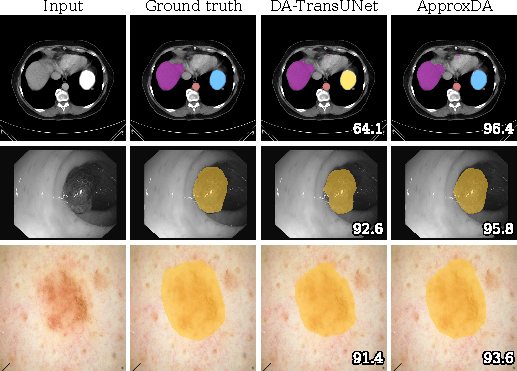
\includegraphics[width=\columnwidth]{figures/fig_qualitative_cross_task.pdf}
  \caption{Qualitative comparison on Synapse (top), CVC-ClinicDB (middle) and ISIC 2018 (bottom). Synapse: a slice where ApproxDA-TransUNet improves most over DA-TransUNet; CVC-ClinicDB and ISIC 2018: the test case with the median ApproxDA-TransUNet DSC. Numbers give the per-image DSC (\%).}
  \label{fig:qualitative}
\end{figure}

\subsection{Computational Cost and Parameter Profile}
\label{sec:efficiency}

Table~\ref{tab:efficiency} reports parameter counts and FLOPs of the reported Synapse ($224{\times}224$) and ISIC 2018 ($256{\times}256$) configurations, measured with fvcore on one image for both architectures; one multiply--add is counted as one FLOP, and only modules executed in the forward pass are counted (three attention blocks in DA-TransUNet, four in ApproxDA-TransUNet). Because ApproxDABlocks keep DA-TransUNet's $C/16$ bottleneck and only replace the dense PAM/CAM operators, the attention blocks require 54--57\% fewer FLOPs than DA-TransUNet's dual-attention heads, even though ApproxDA-TransUNet places a fourth block at the $112{\times}112$ skip. Whole-network cost is dominated by the CNN--ViT backbone (the ViT encoder alone accounts for 85.1M parameters), so total FLOPs decrease by only 1.6--1.8\% and parameter counts stay within 1M of DA-TransUNet. ApproxDA-TransUNet is therefore intended as a controlled platform for studying attention approximation rather than as an efficiency-oriented architecture.

\begin{table}[ht]
  \caption{Parameters and FLOPs per Image}
  \label{tab:efficiency}
  \centering
  \setlength{\tabcolsep}{3pt}
  \begin{tabular}{lcccc}
    \toprule
    Method & Input & Params (M) & GFLOPs & Attn.\ GFLOPs \\
    \midrule
    DA-TransUNet~\cite{sun2024datransunet}  & 224 & 106.56 & 30.20 & 0.87 \\
    ApproxDA ($M$=112, $r$=32)              & 224 & 107.50 & 29.73 & 0.40 \\
    \midrule
    DA-TransUNet~\cite{sun2024datransunet}  & 256 & 106.60 & 39.75 & 1.22 \\
    ApproxDA ($M$=64, $r$=32)               & 256 & 106.46 & 39.05 & 0.52 \\
    \bottomrule
  \end{tabular}\par\vspace{3pt}
  \begin{minipage}{\linewidth}\footnotesize Attn.: attention blocks only. ApproxDA: gate=pam.\end{minipage}
\end{table}

% !TEX root = ../ApproxDA-TransUNet.tex
\section{Ablation Studies and Analysis}
\label{sec:understanding}

This section investigates how ApproxDA-TransUNet behaves across approximation parameters and segmentation tasks through systematic ablation studies.

\subsection{Window Size and Rank Ablation}
\label{sec:approx_scale}

We first examine how spatial window size and projection rank govern segmentation performance. Table~\ref{tab:window_ablation} crosses the window size $M{\in}\{7,28,56,112\}$ with low-rank ($r{=}32$) and exact ($r{=}0$) attention under gate=pam and $G{=}8$ on Synapse, and varies the rank at $M{=}112$. $M{=}112$ gives every feature map map-wide spatial scope; with $r{=}0$ it is full (exact) position attention.

\begin{table}[ht]
  \caption{Window Size and Rank Ablation on Synapse}
  \label{tab:window_ablation}
  \centering
  \setlength{\tabcolsep}{4pt}
  \small
  \begin{tabular}{ccc}
    \toprule
    $M$ & Low-rank, $r{=}32$ & Exact, $r{=}0$ \\
    \midrule
    7   & \underline{79.92} / 21.56 & 79.35 / 24.16 \\
    28  & 79.16 / 27.30 & 78.70 / 20.83 \\
    56  & 79.46 / 21.06 & 79.61 / 20.92 \\
    112 & \textbf{81.63} / 23.73 & 79.04 / \textbf{18.22} \\
    \midrule
    112 & $r{=}16$: 78.71 / 25.53 & $r{=}64$: \underline{79.92} / 23.49 \\
    \bottomrule
  \end{tabular}\par\vspace{3pt}
  \begin{minipage}{\linewidth}\footnotesize DSC (\%) / HD95 (mm). gate=pam, $G{=}8$.\end{minipage}
\end{table}

On Synapse, the best accuracy is obtained with map-wide low-rank attention ($M{=}112$: 81.63\%), while the windowed settings $M{\in}\{7,28,56\}$ stay within 79.16--79.92\%, giving a 2.47\,pp DSC spread across window sizes. Exact attention is not more accurate than its low-rank counterpart at any window size (largest gain $+$0.15\,pp at $M{=}56$), although it yields lower HD95 at $M{=}28$ and $M{=}112$. Rank variation at $M{=}112$ is non-monotonic ($r{=}16/32/64$: 78.71/81.63/79.92\%); in this single-seed sweep, exact attention therefore offers no accuracy advantage over the low-rank approximation.

\subsection{Cross-task Ablation and Global Context Sensitivity}
\label{sec:obs2}

\begin{figure}[!t]
\centering
\scalebox{1.0}{%
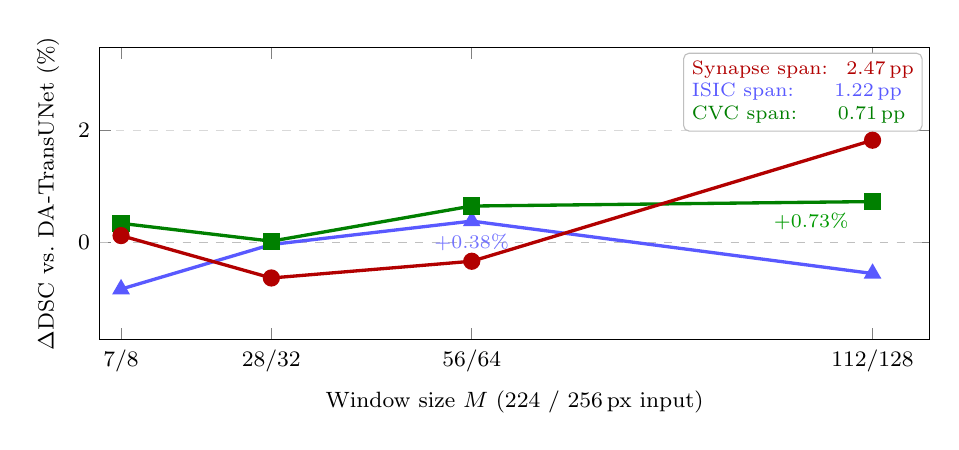
\begin{tikzpicture}
\begin{axis}[
  width=\columnwidth, height=5.3cm,
  xlabel={Window size $M$ (224 / 256\,px input)},
  ylabel={$\Delta$DSC vs.\ DA-TransUNet (\%)},
  ymin=-1.75, ymax=3.5,
  xtick={7,28,56,112},
  xticklabels={7/8,28/32,56/64,112/128},
  xmin=4, xmax=120,
  ymajorgrids=true,
  grid style={dashed,gray!30},
  tick label style={font=\footnotesize},
  label style={font=\footnotesize},
  every axis plot/.append style={very thick, mark size=2.5pt},
]
% Zero reference
\addplot[dashed, gray!50, very thin, forget plot] coordinates {(4,0)(120,0)};
% ISIC 2018 (drawn first, behind); 256 px input, M in {8,32,64,128} plotted at the same relative scale
\addplot[color=blue!65, mark=triangle*]
  coordinates {(7,-0.84) (28,-0.04) (56,0.38) (112,-0.56)};
% CVC-ClinicDB (drawn second); 256 px input like ISIC, values relative to the reported DA-TransUNet (89.47)
\addplot[color=green!50!black, mark=square*]
  coordinates {(7,0.34) (28,0.02) (56,0.65) (112,0.73)};
% Synapse (drawn last — on top of all other lines)
\addplot[color=red!70!black, mark=*]
  coordinates {(7,0.12) (28,-0.64) (56,-0.34) (112,1.83)};
% Peak label — Synapse
\node[font=\scriptsize, color=red!80, anchor=south]
  at (axis cs:112,1.9) {$+$1.83\%};
% Peak label — ISIC (below point to avoid curves above)
\node[font=\scriptsize, color=blue!55, anchor=north]
  at (axis cs:56,0.32) {$+$0.38\%};
% Peak label — CVC-ClinicDB
\node[font=\scriptsize, color=green!60!black, anchor=north east]
  at (axis cs:110,0.70) {$+$0.73\%};
% Span annotation box
\node[anchor=north east, align=left, font=\scriptsize,
      fill=white, draw=gray!50, inner sep=3pt, rounded corners=2pt]
  at (axis cs:119, 3.40) {%
    \textcolor{red!70!black}{Synapse span:\phantom{0} 2.47\,pp}\\
    \textcolor{blue!65}{ISIC span:\phantom{000} 1.22\,pp}\\
    \textcolor{green!50!black}{CVC span:\phantom{000} 0.71\,pp}};
\end{axis}
\end{tikzpicture}}
\caption{$\Delta$DSC relative to DA-TransUNet (Tables~\ref{tab:synapse}--\ref{tab:isic}) vs.\ window size $M$; gate=pam, $r{=}32$.}
\label{fig:dsc_vs_m}
\end{figure}

We next assess whether attention approximation responds consistently across distinct anatomical segmentation tasks. Although ApproxDA-TransUNet employs identical approximation mechanisms across benchmarks, its empirical sensitivity to window selection diverges significantly. On Synapse multi-organ CT, the DSC-vs-$M$ curve (Figure~\ref{fig:dsc_vs_m}) peaks at map-wide attention ($M{=}112$) and spans 2.47\,pp. Conversely, on CVC-ClinicDB the curve is flat (0.71\,pp spread) with an optimum at $M{=}128$; on ISIC 2018, the range across $M{\in}\{8,32,64,128\}$ is 1.22\,pp (at $256{\times}256$ input these windows cover the same fraction of each feature map as $\{7,28,56,112\}$ at $224{\times}224$).
The raw DSC values across the four window sizes (gate=pam, $r{=}32$) are 89.81/89.49/90.12/90.20\% on CVC-ClinicDB and 88.04/88.84/89.26/88.32\% on ISIC 2018. With the best window, ApproxDA-TransUNet exceeds the DA-TransUNet values in Tables~\ref{tab:synapse}--\ref{tab:isic} by $+$1.83\% (Synapse, $M{=}112$), $+$0.73\% (CVC-ClinicDB, $M{=}128$), and $+$0.38\% (ISIC 2018, $M{=}64$).

We formalize this cross-task behavior through the empirical metric \textbf{Global Context Sensitivity (GCS)}, defined as the performance span over the window sweep:
\begin{equation}
  \Delta\text{DSC} = \max_{M} \text{DSC}(M) - \min_{M} \text{DSC}(M),
\end{equation}
measured under uniform gate=pam, $r{=}32$. Empirically, $\Delta\text{DSC} = 2.47$\,pp on Synapse, $0.71$\,pp on CVC-ClinicDB, and $1.22$\,pp on ISIC~2018---a 3.5$\times$ and 2.0$\times$ ratio relative to polyp and lesion segmentation, respectively. Rather than serving as an a priori predictive descriptor, GCS provides a quantified diagnostic of how strongly model accuracy is coupled to spatial context scale. High GCS reflects a sharp optimization landscape requiring careful window tuning, whereas low GCS demonstrates broad stability across receptive scopes. Importantly, high GCS does not indicate that approximation degrades performance, but rather characterizes performance sensitivity to window calibration.

These differences align with the contrasting anatomical context requirements of the tasks. Multi-organ abdominal CT segmentation involves inter-organ spatial dependencies, and map-wide attention gives the best result there. In contrast, polyp and skin lesion segmentation are driven mainly by local texture, color contrast, and boundary continuity, so the window size matters less; on CVC-ClinicDB the channel branch alone even gives the best result (Table~\ref{tab:cvc}).

\subsection{Routing Mechanism Ablation}
\label{sec:collapse}

We analyze branch routing by evaluating PAM-only, CAM-only, fixed equal blending, and learnable gating on Synapse under fixed $M{=}28$, $r{=}32$, $G{=}8$, and the CAM group count $G$ under CAM-only routing (Table~\ref{tab:gate_ablation}).

\begin{table}[ht]
  \caption{Routing and CAM Group Ablation on Synapse}
  \label{tab:gate_ablation}
  \centering
  \setlength{\tabcolsep}{4pt}
  \small
  \begin{tabular}{llcc}
    \toprule
    Gate Mode & $\mathbf{g}$ & DSC (\%) $\uparrow$ & HD95 (mm) $\downarrow$ \\
    \midrule
    gate=pam   & $\mathbf{1}$              & 79.16 & 27.30 \\
    gate=cam   & $\mathbf{0}$              & 79.34 & 26.03 \\
    gate=fixed & $0.5\cdot\mathbf{1}$      & 79.27 & \textbf{21.27} \\
    gate=learn & ${\approx}0.5\cdot\mathbf{1}^*$ & 78.96 & \underline{21.48} \\
    \midrule
    gate=cam, $G{=}1$ & $\mathbf{0}$ & \underline{80.03} & 23.62 \\
    gate=cam, $G{=}4$ & $\mathbf{0}$ & \textbf{80.10} & 22.54 \\
    \bottomrule
  \end{tabular}\par\vspace{3pt}
  \begin{minipage}{\linewidth}\footnotesize $M{=}28$, $r{=}32$; $G{=}8$ unless stated. $^*$Learned; stays near 0.5.\end{minipage}
\end{table}

% figures/fig_entropy_scatter.pdf (vector): experiments/ApproxDA-TransUNet/analyze_gate_entropy.py (Fig B) on the M=28 learned-gate run, epoch 300
\begin{figure}[ht]
  \centering
  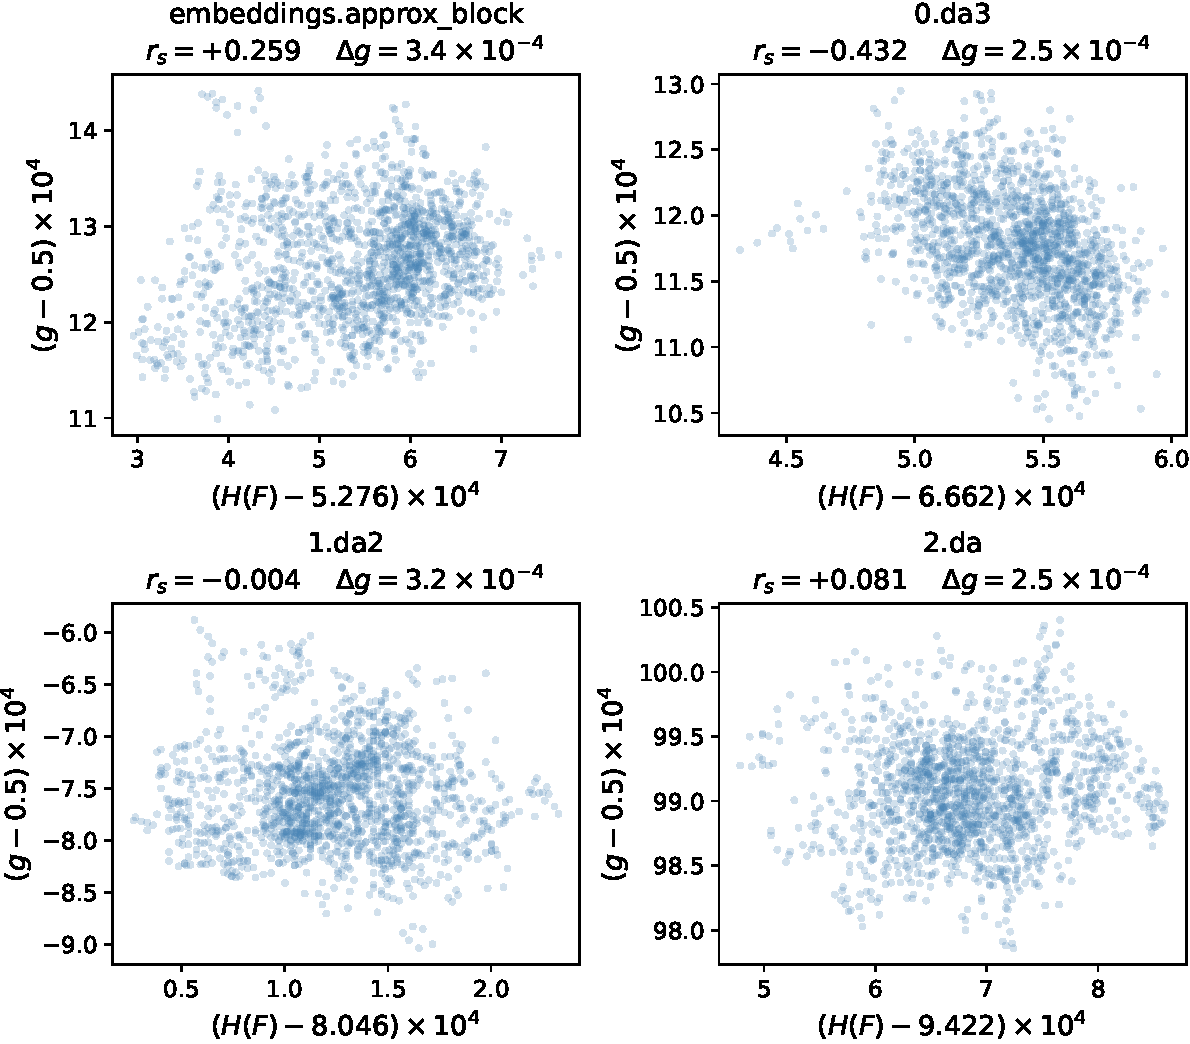
\includegraphics[width=\columnwidth]{figures/fig_entropy_scatter.pdf}
  \caption{Mean gate $g$ vs.\ input feature entropy $H(F)$ per Synapse test slice at the bottleneck and the 28$^2$, 56$^2$ and 112$^2$ skips ($M{=}28$, gate=learn).}
  \label{fig:gate_analysis}
\end{figure}

The four routing modes lie within 0.38\,pp DSC (78.96--79.34\%), and the learnable gate does not outperform single-branch routing; blending both branches (fixed or learned) mainly lowers HD95. Within CAM-only routing, fewer groups give slightly higher DSC ($G{=}1/4/8$: 80.03/80.10/79.34\%). In our Synapse experiments, the learnable gate stayed at a near-uniform state ($g \approx 0.5$) throughout training: over 300 epochs, the block-mean gate of all four ApproxDABlocks remained within 0.499--0.512, the spread of per-channel means was at most 0.022 (standard deviation), and the median variation across samples was $4{\times}10^{-4}$. On the test slices (Figure~\ref{fig:gate_analysis}), the per-slice mean gate varies by at most $3.4{\times}10^{-4}$ at every block and has no consistent relation to the entropy of the block input (Spearman $r_s$ between $-0.43$ and $+0.26$). We document this as an empirical phenomenon and do not analyze its cause here; alternative gate initializations and regularization are left to future work. Because routing changes DSC little on Synapse, PAM-only routing serves as the standard configuration for the window ablations. On CVC-ClinicDB, in contrast, CAM-only routing with $G{=}1$ gives the highest DSC (90.54\%, Table~\ref{tab:cvc}), whereas the learned gate (89.90\%) again does not outperform single-branch routing.

% !TEX root = ../ApproxDA-TransUNet.tex
\section{Conclusion}
\label{sec:conclusion}
This paper presented ApproxDA-TransUNet, a dual-attention approximation framework for medical image segmentation featuring independently controllable window size, projection rank, and channel grouping. Across three representative clinical benchmarks, ApproxDA-TransUNet improves Dice over the reported DA-TransUNet results with appropriately selected configurations, showing that the choice of attention approximation affects accuracy rather than acting solely as an efficiency mechanism.

Our systematic ablations further show that window sensitivity differs substantially across clinical targets: multi-organ CT segmentation is considerably more sensitive to window scale and benefits from map-wide context, whereas polyp and skin-lesion segmentation is more robust across receptive scopes. Exact attention shows no consistent advantage over the low-rank approximation. In addition, learnable dual-branch routing stays at near-uniform blending on multi-organ CT without surpassing single-branch routing.

\textbf{Limitations and Future Work.} Two limitations remain. First, the mechanism behind this window sensitivity is not yet understood: the DSC span summarizes how accuracy responds to the window size on the evaluated benchmarks, but why some targets benefit from map-wide context, and whether this can be predicted before an exhaustive sweep, remains open and needs validation across broader anatomical modalities and architectures. Second, the CNN--ViT backbone dominates the computational cost, so the savings of the approximated attention barely reach the whole network; lightweight backbones and specialized attention kernels are needed to turn them into end-to-end efficiency gains. We hope this work encourages principled, task-aware exploration of attention approximation across medical imaging domains.


\bibliographystyle{IEEEtran}
\bibliography{references}
\end{document}
